\documentclass[twoside, 11pt, a4paper]{article}
\usepackage{amsmath,amsfonts,amssymb,graphicx,parskip}
\usepackage[utf8]{inputenc}
\usepackage{subfigure}

\DeclareMathOperator{\eps}{\epsilon}
\newcommand{\dee}{\mathrm{d}}

\title{Spalart-Allmaras turbulence model - IFEM implementation}
\author{Arne Morten Kvarving}
\begin{document}
\maketitle

This document describe the derivation of the weak form, and the associated
Jacobian, for the Spalart-Allmaras turbulence model given in \cite{sa}.
It is implemented in SplineFEM in the SpalartAllmaras
Integrand, see src/Integrands/SpalartAllmaras.h/C, while
you can find a test application (and SIM classes) in Apps/SpalartAllmaras.

\section{Equations}

Initial expression:
\begin{equation}
	\frac{\partial\tilde{\nu}}{\partial t} + \mathbf{u}\cdot\nabla\tilde{\nu} = c_{b1}\tilde{S}\tilde{\nu}+\frac{1}{\sigma}\left(\nabla\cdot\left(\nu + \tilde{\nu}\right)\nabla\tilde{\nu} + c_{b2}\left|\nabla\tilde{\nu}\right|^2\right) - c_{w1}f_w\left(\frac{\tilde{\nu}}{d}\right)^2.
\end{equation}
Here $\tilde{S}$ models the production and is given by
\begin{equation}
	\tilde{S} = S + \frac{\tilde{\nu}}{k^2d^2}f_{\tilde{\nu}2}
\end{equation}
where $S$ is the normal strain tensor
\begin{equation}
	\begin{split}
		S &\equiv \sqrt{\hat{\Omega}_{ij}\hat{\Omega}_{ij}}, \\
		\hat{\Omega}_{ij} &\equiv \partial_j u_i - \partial_i u_j, \\
		X &= \frac{\tilde{\nu}}{\nu}, \\
		f_{\tilde{\nu}1} &= \frac{X^3}{X^3+c_{\tilde{\nu}1}^3}, \\
		f_{\tilde{\nu}2} &= 1-\frac{X}{1+Xf_{\tilde{\nu}1}}, \\
		c_{\tilde{\nu}1} &= 7.1, \\
		c_{b1} &= 0.1355, \\
		k &= 0.41.
	\end{split}
\end{equation}

The center terms models the diffusion. Here
\begin{equation}
	\sigma = \frac{2}{3},\ c_{b2} = 0.622
\end{equation}

Finally, the last term models destruction. Here
\begin{equation}
	\begin{split}
		f_w = g\left[\frac{1+c_{w3}^6}{g^6+c_{w3}^3}\right]^{1/6}; \quad g = r + c_{w2}\left(r^6-r\right); \quad r \equiv \frac{\tilde{\nu}}{\tilde{S}k^2d^2} \\
		c_{w1} = c_{b1}/k^2+(1+c_{b2})/\sigma,\quad c_{w2} = 0.3,\quad c_{w3} = 2.
	\end{split}
\end{equation}

Furthermore, we have that $\hat{\Omega}_{ij} \equiv \partial_j u_i-\partial_i u_j$.
That is
\[
  \hat{\Omega}  = \begin{bmatrix}
                    0 & \frac{1}{2}\left(\frac{\partial u_1}{\partial x_2}-\frac{\partial u_2}{\partial x_1}\right) & \frac{1}{2}\left(\frac{\partial u_1}{\partial x_3}-\frac{\partial u_3}{\partial x_1}\right) \\
                    \frac{1}{2}\left(\frac{\partial u_2}{\partial x_1}-\frac{\partial u_1}{\partial x_2}\right) & 0 & \frac{1}{2}\left(\frac{\partial u_2}{\partial x_3}-\frac{\partial u_3}{\partial x_2}\right) \\
                    \frac{1}{2}\left(\frac{\partial u_3}{\partial x_1}-\frac{\partial u_1}{\partial x_3}\right) & \frac{1}{2}\left(\frac{\partial u_3}{\partial x_2}-\frac{\partial u_2}{\partial x_3}\right) & 0
                  \end{bmatrix} =
                  \begin{bmatrix}
                     0 & a & b \\
                    -a & 0 & c \\
                    -b & -c & 0
                  \end{bmatrix}
\]
Thus,
\[
  \hat{\Omega}\hat{\Omega}  = 2a^2+2b^2+2c^2
\]
and
\[
  S = 2\sqrt{a^2+b^2+c^2}.
\]

\subsection*{Derivation of the Jacobian}
Temporal term: In this case we consider a BDF1 discretization.

\subsubsection*{Advection term}
\bf Strong form:\rm
\begin{equation}
  \mathbf{u}\cdot\nabla\delta\nu
\end{equation}
The weak form is straight forward.

\subsubsection*{Production term}
\bf Strong from:\rm
\begin{equation}
  c_{b1}\hat{S}\delta\nu
\end{equation}
The weak form gives a simple mass term.

\subsubsection*{Diffusion terms}
\bf Strong form:\rm
\begin{equation}
  \frac{1}{\sigma}\left(\nabla\cdot\left(\nu+\tilde{\nu}+\delta\nu\right)\nabla\left(\tilde{\nu}+\delta\nu\right)+c_{b2}\left|\nabla\tilde{\nu}+\nabla\delta\nu\right|^2\right)
\end{equation}
\bf Linearized, first term:\rm
\begin{equation}
  \nabla\cdot\nu\nabla\delta\nu + \nabla\cdot\tilde{\nu}\nabla\delta\nu + \nabla\cdot\delta\nu\nabla\tilde{\nu}.
\end{equation}
\bf Linearized, second term:\rm
\begin{equation}
  2\nabla\tilde{\nu}\cdot\nabla\delta\nu
\end{equation}

\bf Weak form, first term:\rm
\begin{equation}
  \begin{aligned}
    \int_\Omega \nabla \cdot \left(\nu\nabla\delta\nu + \tilde{\nu}\nabla\delta\nu + \delta\nu\nabla\tilde{\nu}\right)v\,\dee\Omega &=&
    \int_{\partial\Omega} \left(\nu\nabla\delta\nu + \tilde{\nu}\nabla\delta\nu + \delta\nu\nabla\tilde{\nu}\right)v\cdot \mathbf{n}\,\dee S \\
    &-&\int_\Omega \left(\nu\nabla\delta\nu + \tilde{\nu}\nabla\delta\nu + \delta\nu\nabla\tilde{\nu}\right)\cdot \nabla v\,\dee\Omega.
   \end{aligned}
\end{equation}

\bf Weak form, second term:\rm \\
Straight forward, no integration by parts have to be performed.
\newpage

\section{Verification}
We have performed some verification studies to confirm that the model 

The first one is a two-dimensional backward facing step with a sharp step. The grid and
geometry definition can be found in Figure \ref{fig:bfsgrid}.

\begin{figure}[h]
    \begin{center}
        \includegraphics[width=14cm]{bfs2dgrid}
    \end{center}
    \caption{The geometry (and) grid used for BFS2D code validation test. The grid consists of 18751 nodes.}
    \label{fig:bfsgrid}
\end{figure}

The boundary conditions for the velocity and pressure are given in Figure \ref{fig:bfsupbc}.
\begin{figure}[h]
    \begin{center}
        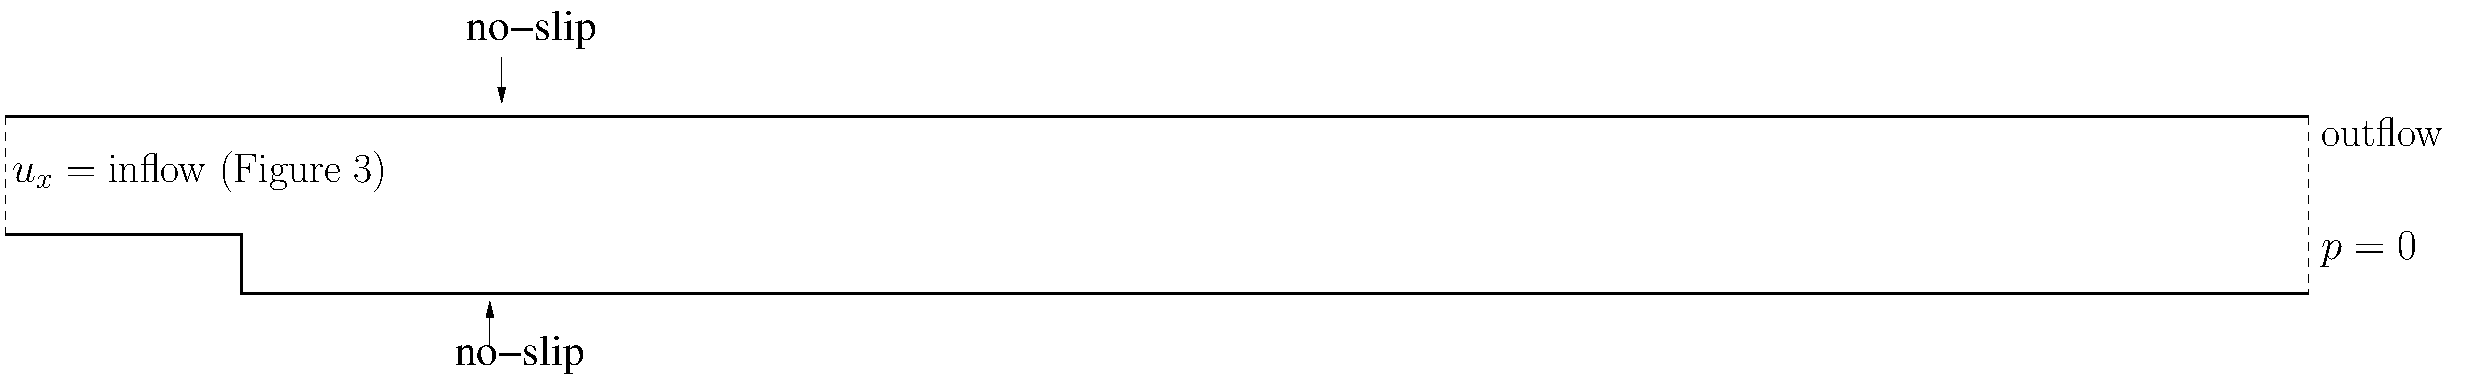
\includegraphics[width=14cm]{bfs2dupbc}
    \end{center}
    \caption{The boundary conditions for the velocity and pressure in the BFS2D code validation test.}
    \label{fig:bfsupbc}
\end{figure}
\begin{figure}[h]
    \begin{center}
        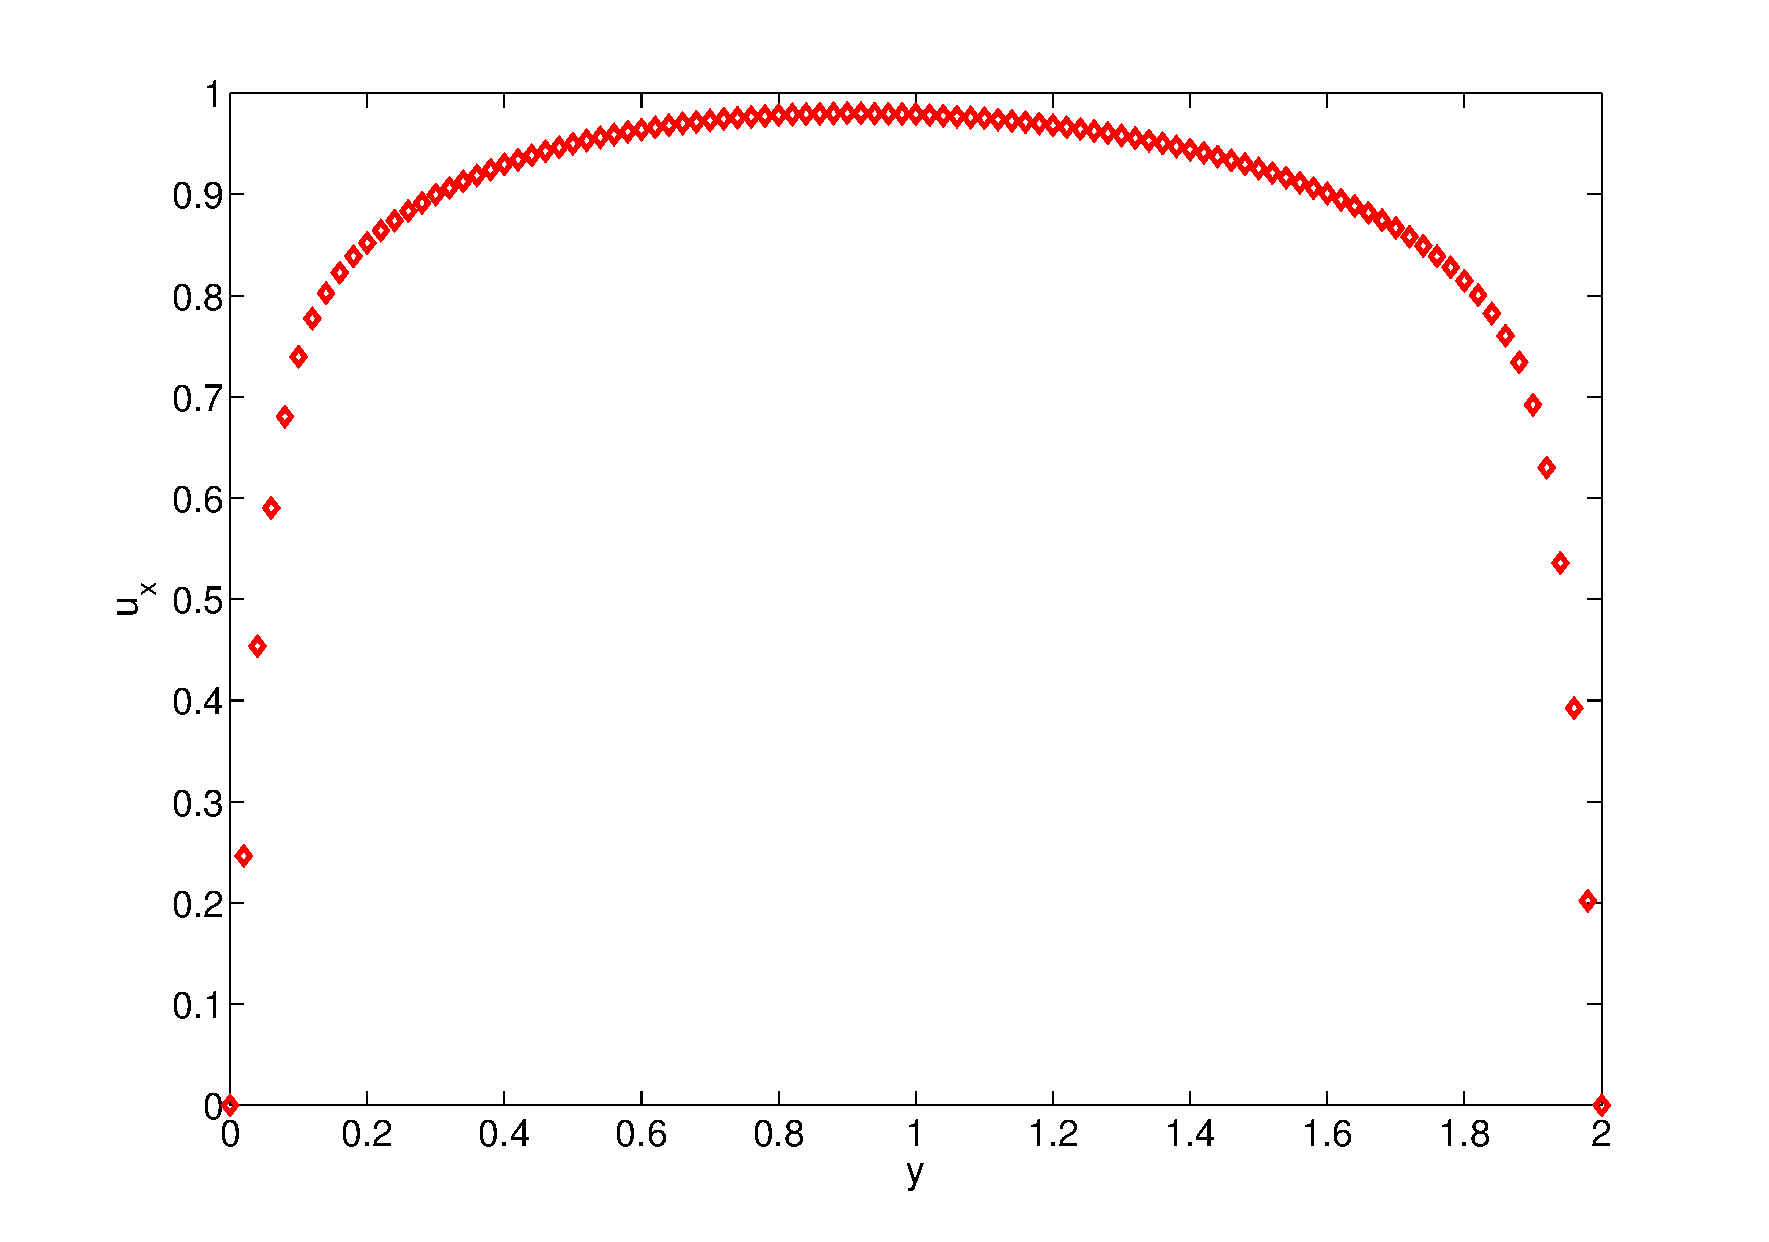
\includegraphics[width=8cm]{inflow}
    \end{center}
    \caption{The inflow velocity profile.}
    \label{fig:bfsinflow}
\end{figure}
The boundary conditions for the turbulent viscosity are given in Figure \ref{fig:bfsnutbc}.
\begin{figure}[h]
    \begin{center}
        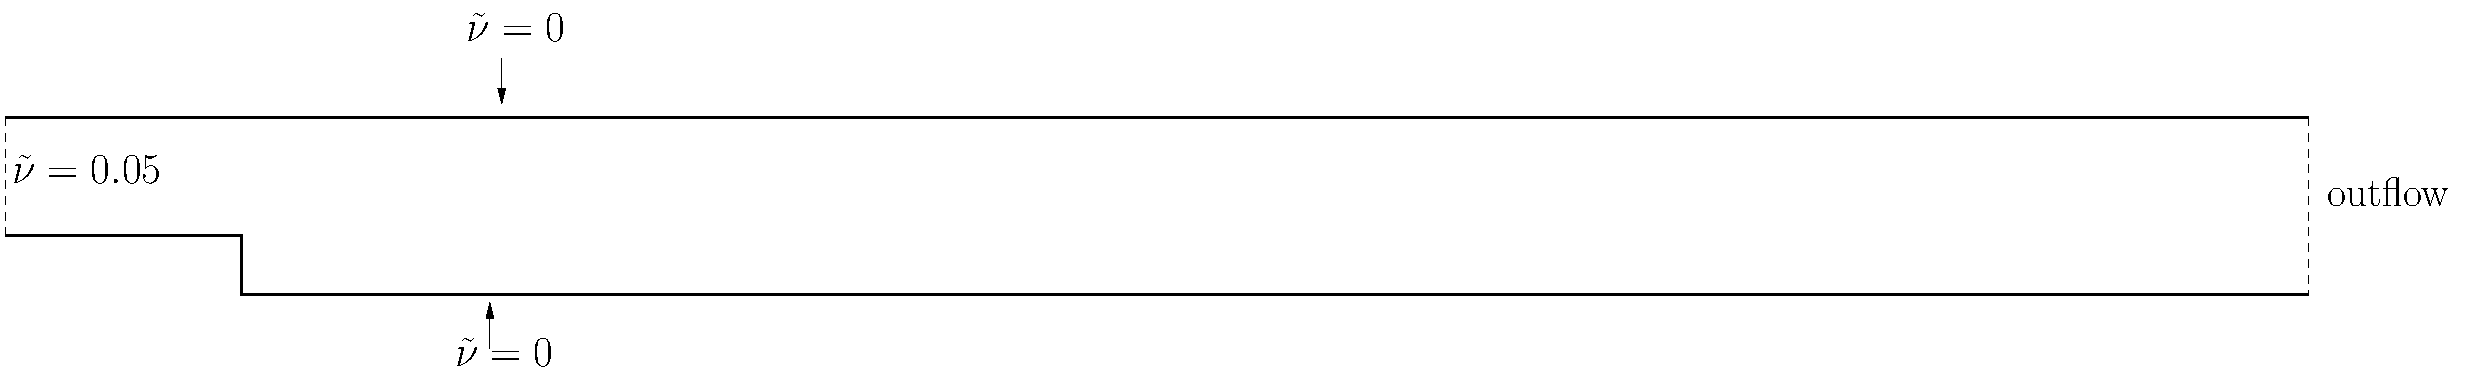
\includegraphics[width=14cm]{bfs2dnutbc}
    \end{center}
    \caption{The boundary conditions for the turbulent viscosity in the BFS2D code validation test.}
    \label{fig:bfsnutbc}
\end{figure}

Some important parameters;
\[
    \begin{split}
        u_{\infty} &= 1 \\
        \nu &= 0.000331 \\
        \rho &= 1 \\
        Re &= 3025 \\
        \Delta t &= 0.005
    \end{split}
\]

The following results were obtained using a second order scheme with SUPG stabilization for both the
turbulence model and the velocity solver. No substantial differences compared to the results without
can be observed using the naked eye.
\newpage
\begin{figure}[h]
    \begin{center}
        \subfigure[$\frac{x}{S}=4$]{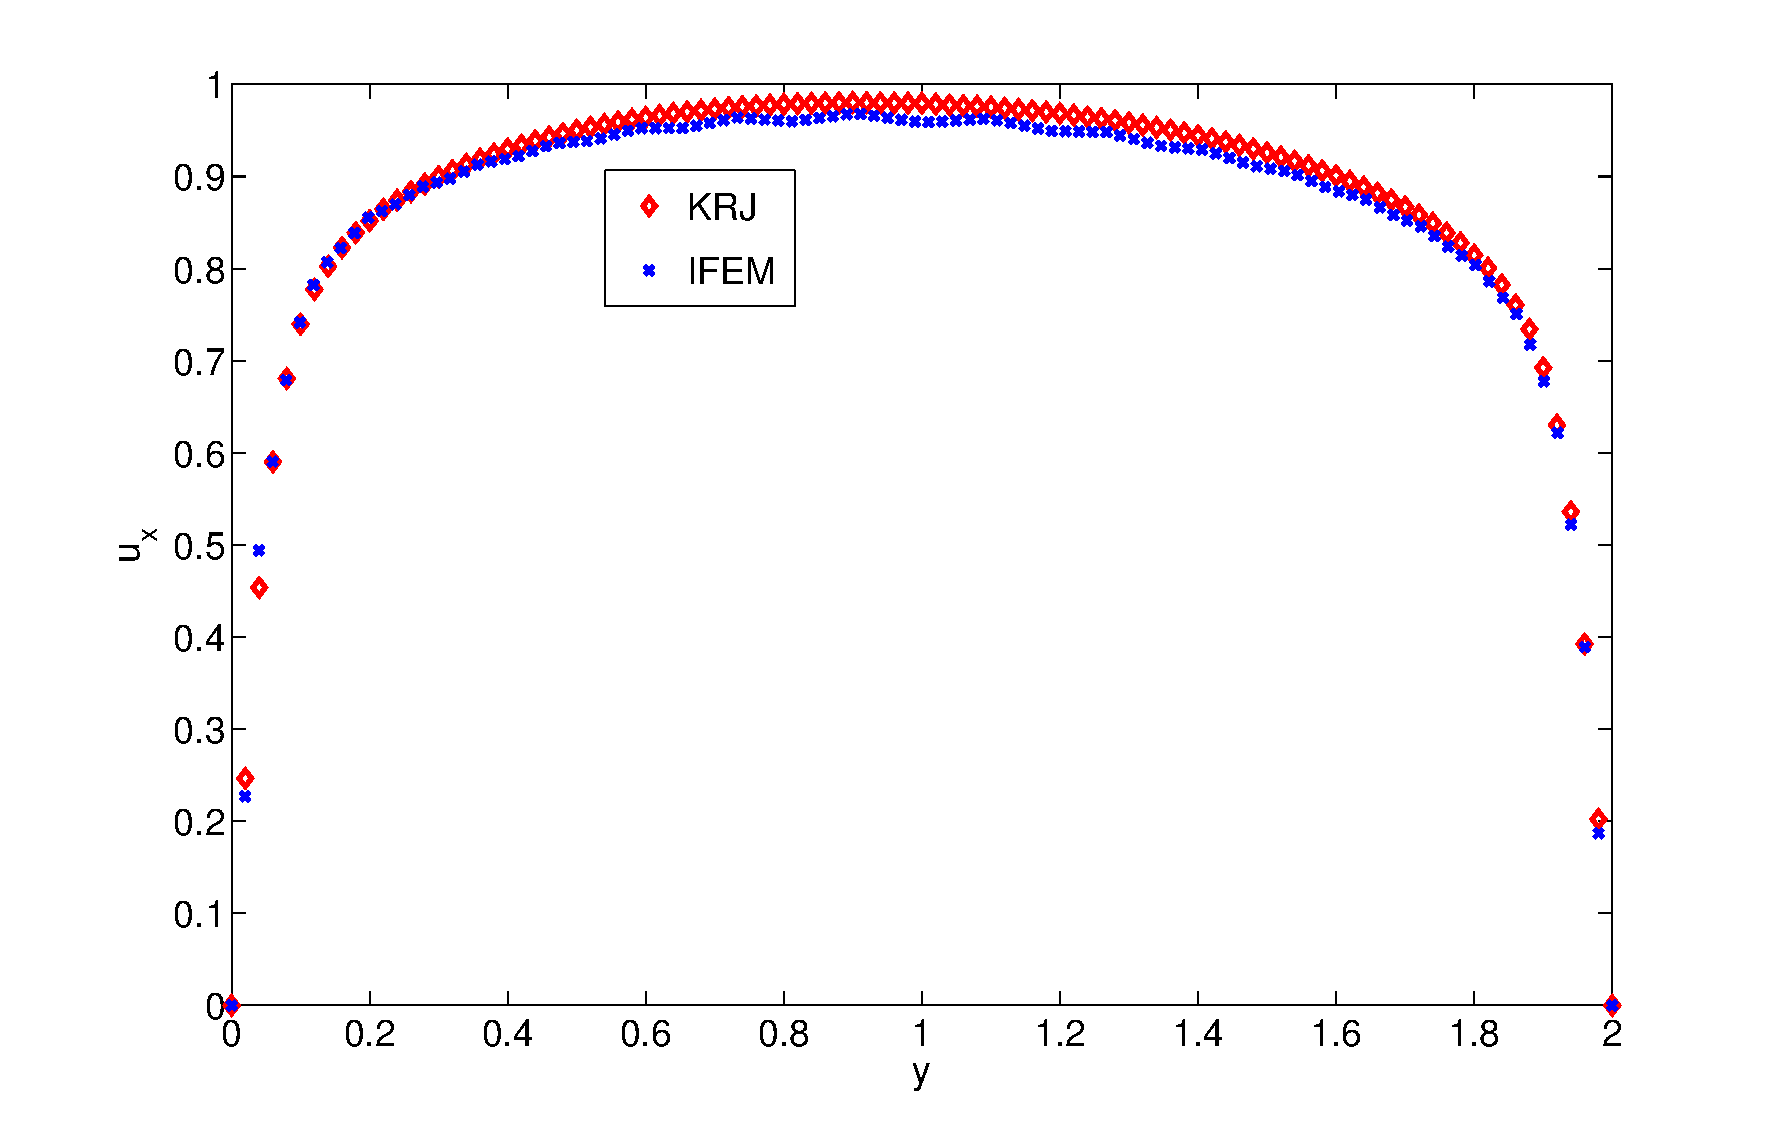
\includegraphics[width=5.5cm]{x0}}
        \subfigure[$\frac{x}{S}=6$]{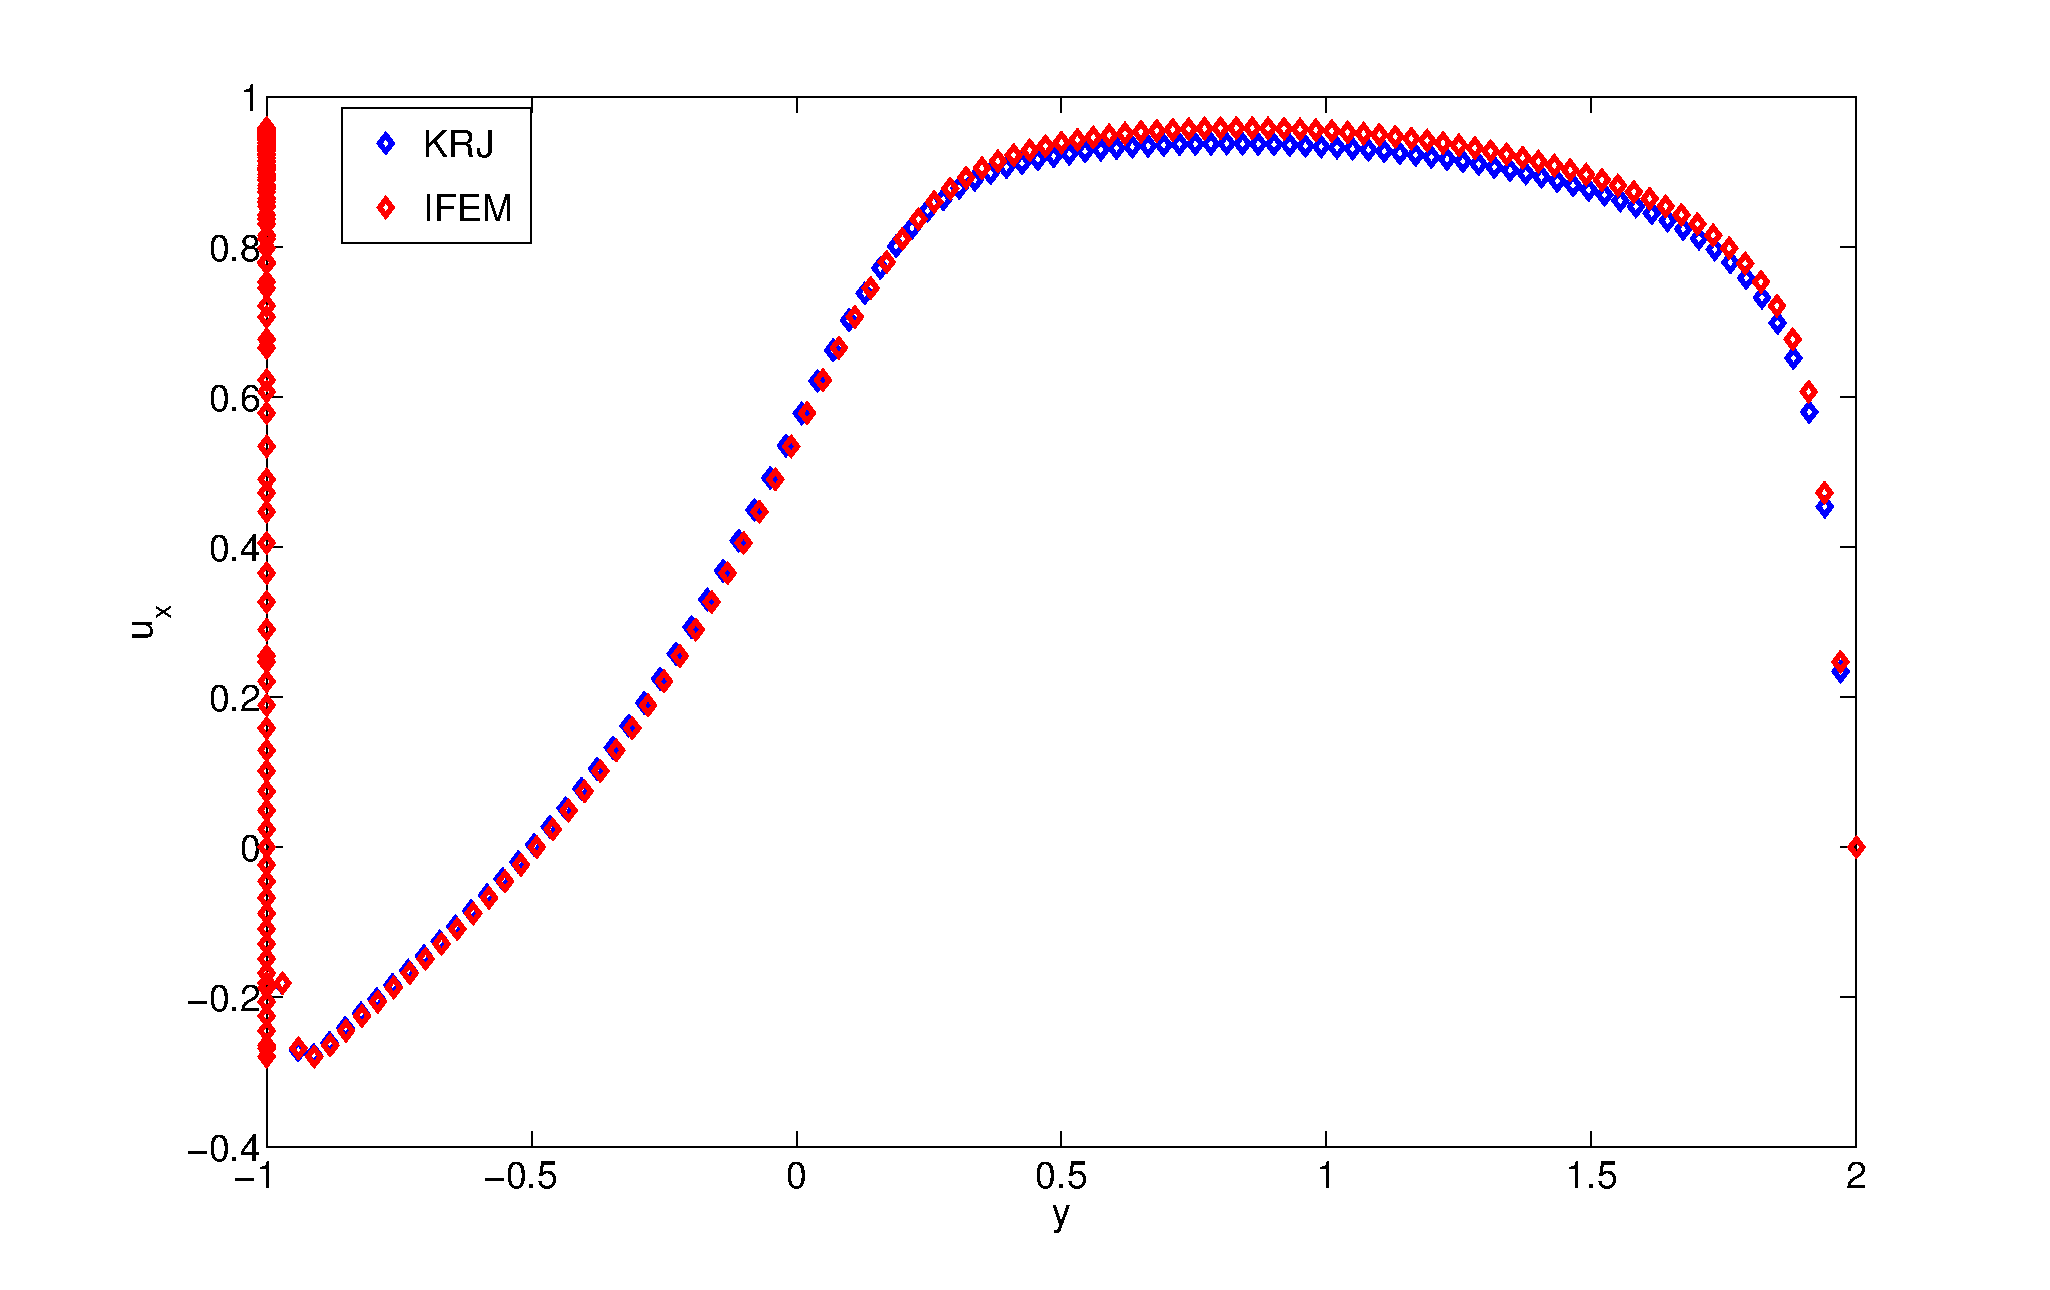
\includegraphics[width=5.5cm]{x2}}
        \subfigure[$\frac{x}{S}=8$]{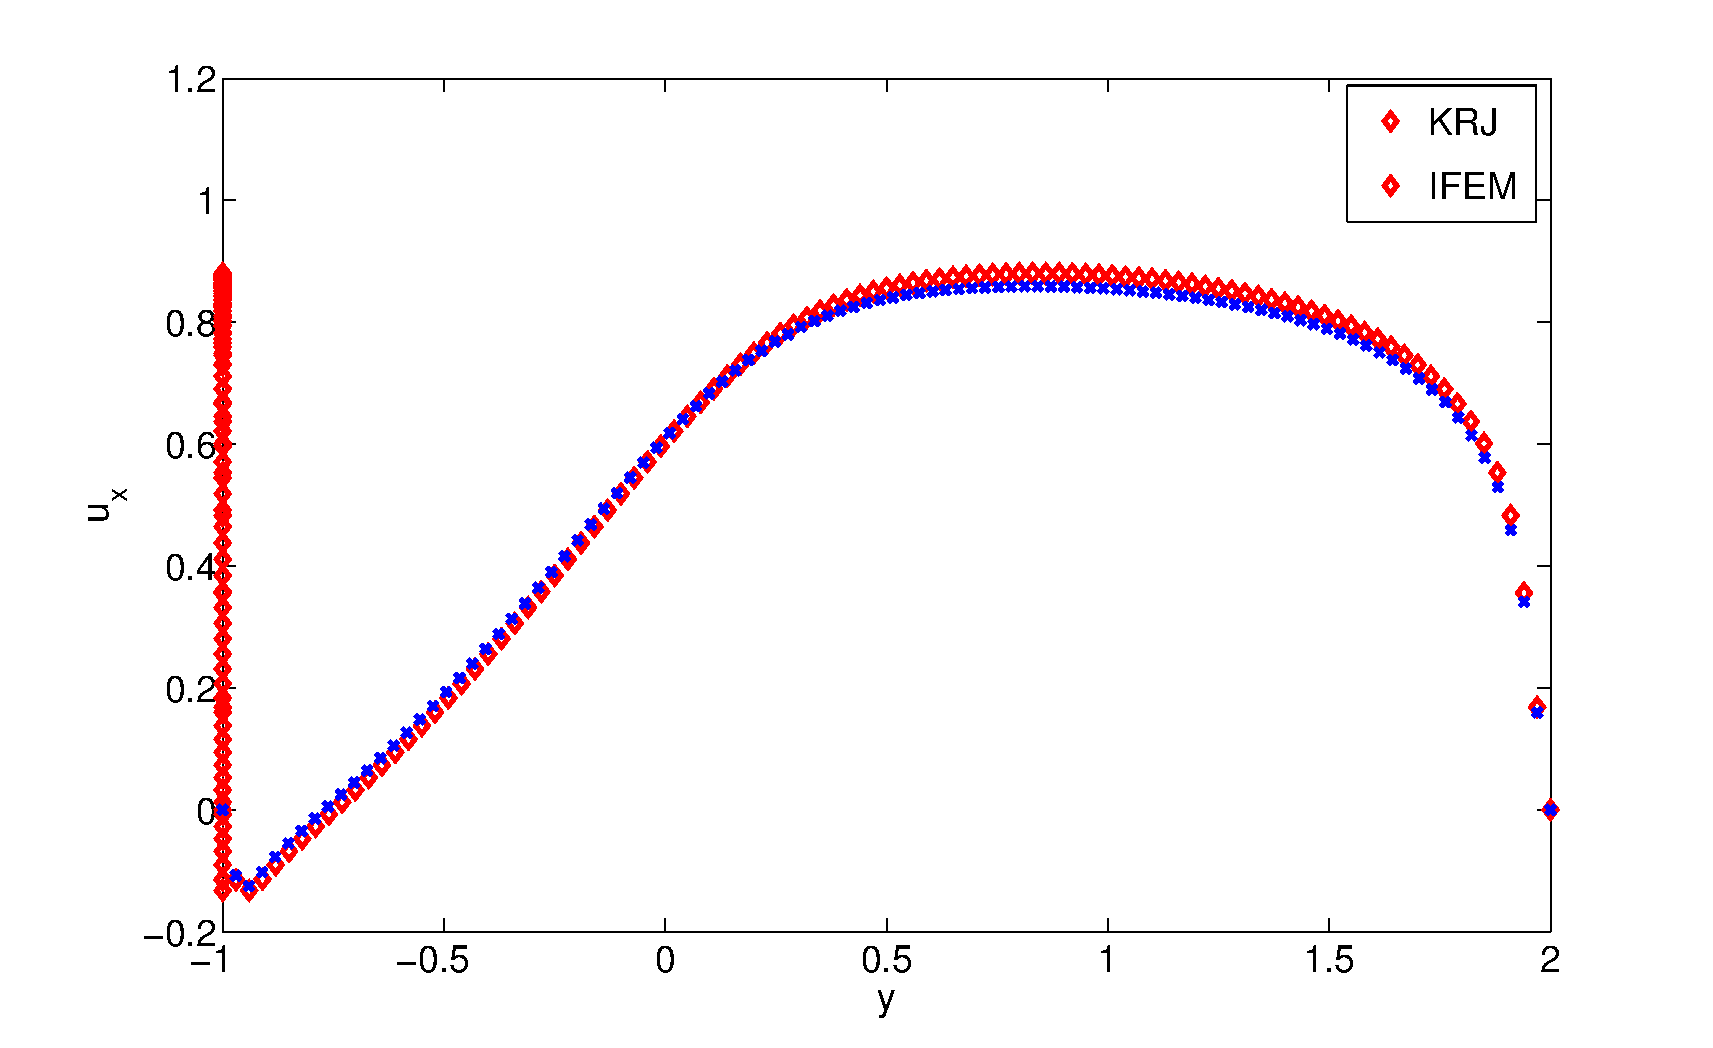
\includegraphics[width=5.5cm]{x4}}
        \subfigure[$\frac{x}{S}=10$]{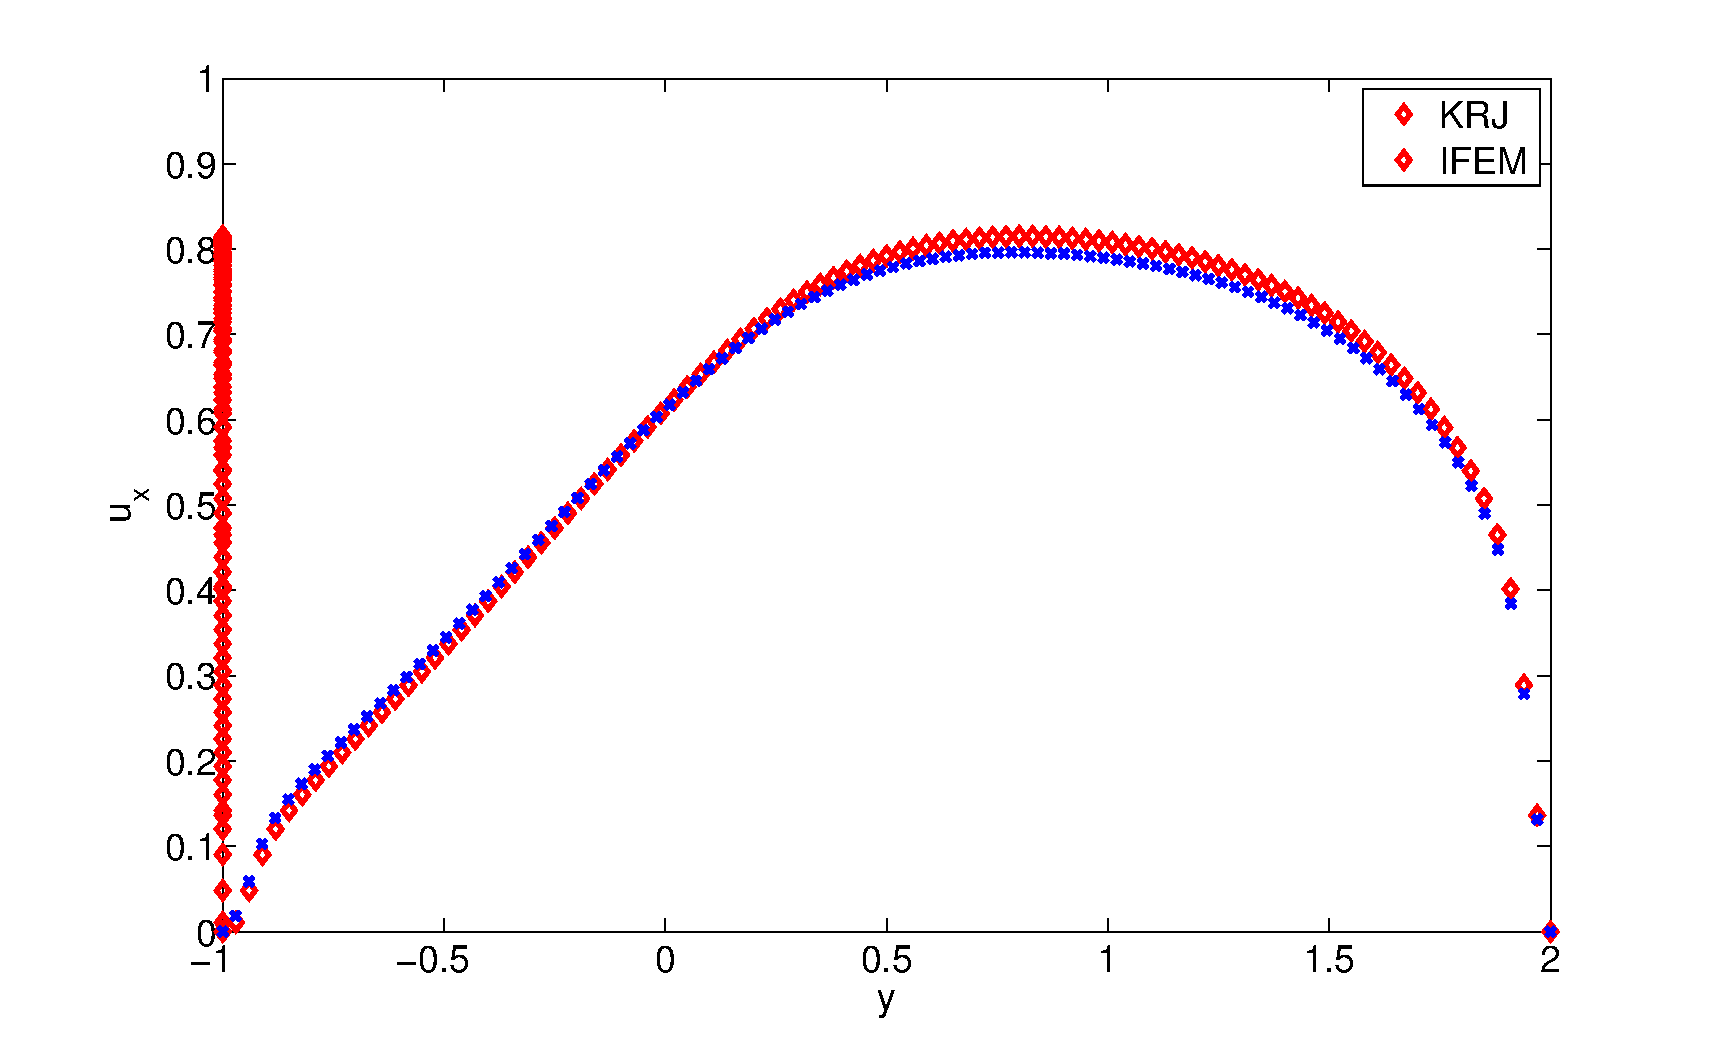
\includegraphics[width=5.5cm]{x6}}
        \subfigure[$\frac{x}{S}=12$]{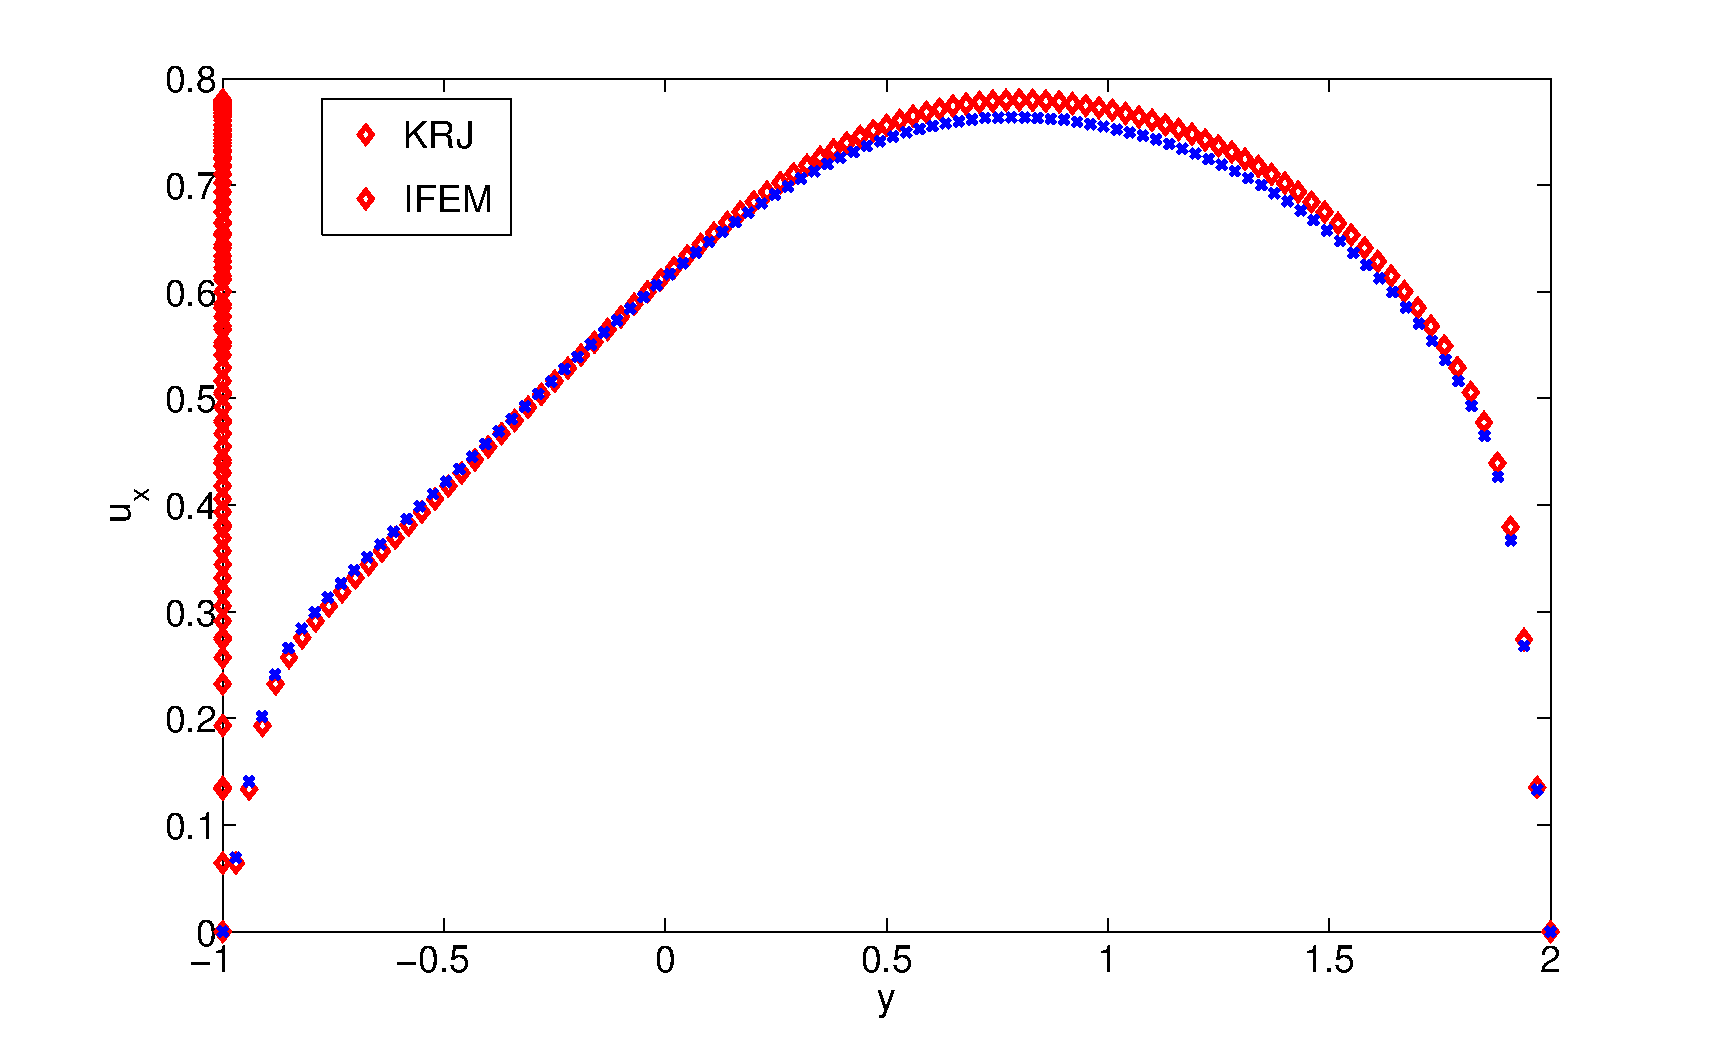
\includegraphics[width=5.5cm]{x8}}
        \subfigure[$\frac{x}{S}=16$]{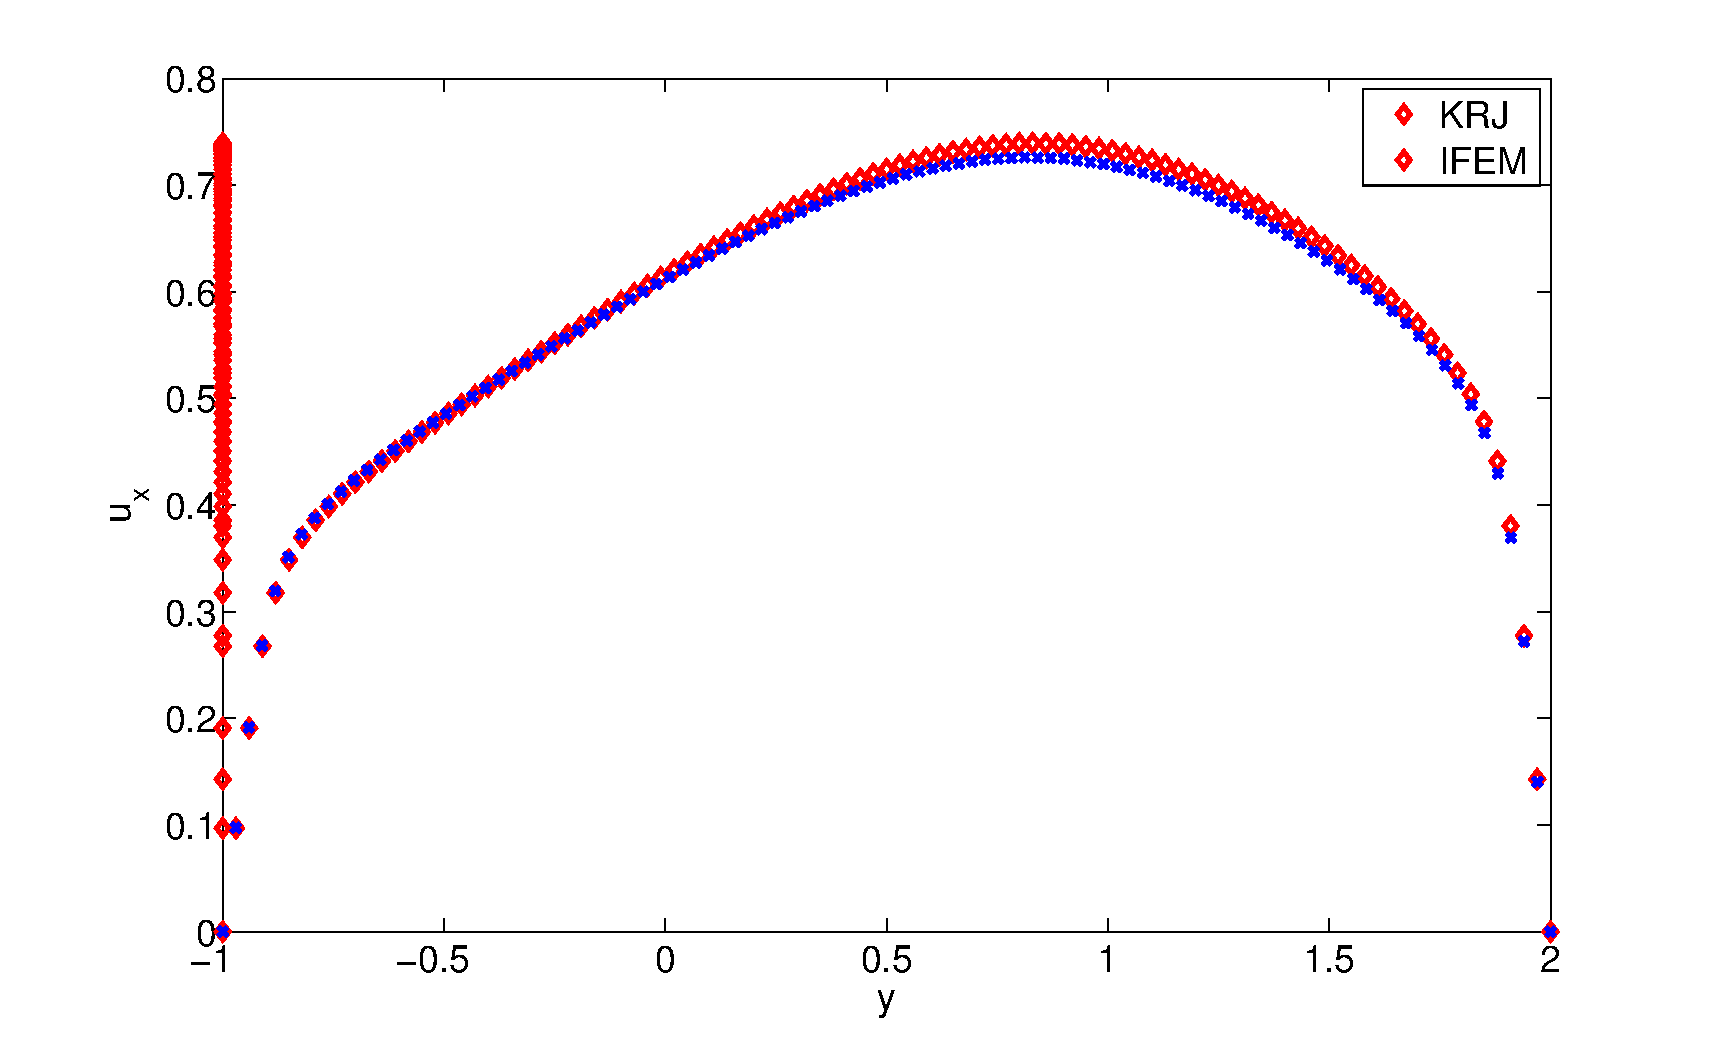
\includegraphics[width=5.5cm]{x12}}
    \end{center}
    \caption{Comparison of velocity profiles.}
    \label{fig:bfsx1}
\end{figure}

\end{document}

